\documentclass[12pt, a4paper]{report}
\usepackage[utf8]{inputenc}
\usepackage[T1]{fontenc}
\usepackage{hyperref}
\hypersetup{colorlinks=true, linkcolor=blue, filecolor=magenta, urlcolor=cyan,}
\urlstyle{same}
\usepackage{amsmath}
\usepackage{amsfonts}
\usepackage{amssymb}
\usepackage{graphicx}
\usepackage{enumitem}
\usepackage{geometry}
\usepackage[export]{adjustbox}
\usepackage{titlesec}
\geometry{lmargin=30mm}
\titleformat{\chapter}{\normalfont\huge}{\thechapter}{20pt}{\huge\bf}
\graphicspath{{images/}} %configuring the graphicx package
\title{Practica 1}
\author{Javier Izquierdo Hernández}
\date{\today}

\begin{document}
	\begin{titlepage}
		\centering
		{
\includegraphics[width=0.3\textwidth]{logo}\par}
		\vspace{1cm}
		{\bfseries\LARGE Universidad Rey Juan Carlos \par}
		\vspace{1cm}
		{\scshape\Large E.T.S. Ingeniería de Telecomunicación \par}
		\vspace{3cm}
		{\scshape\Huge Fundamentos de redes de ordenadores \par}
		\vspace{3cm}
		{\itshape\Large Práctica 5 \par}
		\vfill
		{\Large Autor: \par}
		{\Large Javier Izquierdo Hernández \par}
		\vfill
		{\Large \today \par}
	\end{titlepage}

\newpage
\renewcommand{\contentsname}{Contenidos}
\tableofcontents
\newpage

\chapter{Comunicación de aplicaciones usando el protocolo UDP}
\section{Análisis de captura de tráfico UDP}
En la captura udp.cap se muestra una comunicación UDP. Contesta a las siguientes preguntas:

\begin{enumerate}
	\item ¿Cuáles son las direcciones IP y puertos involucrados en la comunicación?
	
	Son Ip: 10.0.0.2 y Puerto: 32768 ;e Ip: 11.0.0.2 y Puerto: 33000
	
	\item ¿Cuál es el número de paquetes UDP intercambiados? ¿Y número de bytes de datos intercambiados?
	
	Se han intercambiado 2 paquetes UDP, y el numero de bytes intercambiados es 11 bytes
	
\end{enumerate}

\section{Estudio de UDP mediante aplicaciones cliente y servidor lanzadas con nc}
Descarga de la página de la asignatura el fichero lab-p5.tgz, que contiene un escenario de red:

\href{https://mobiquo.gsyc.urjc.es/practicas/fro/p5.html}{https://mobiquo.gsyc.urjc.es/practicas/fro/p5.html}

Descomprímelo de la misma manera que hiciste en prácticas anteriores.

Lanza ahora NetGUI. En el menú, elige File $\rightarrow$ Open y selecciona la carpeta lab-p5 en la que está el escenario. Verás aparecer la red de la figura 1.

\begin{center}
	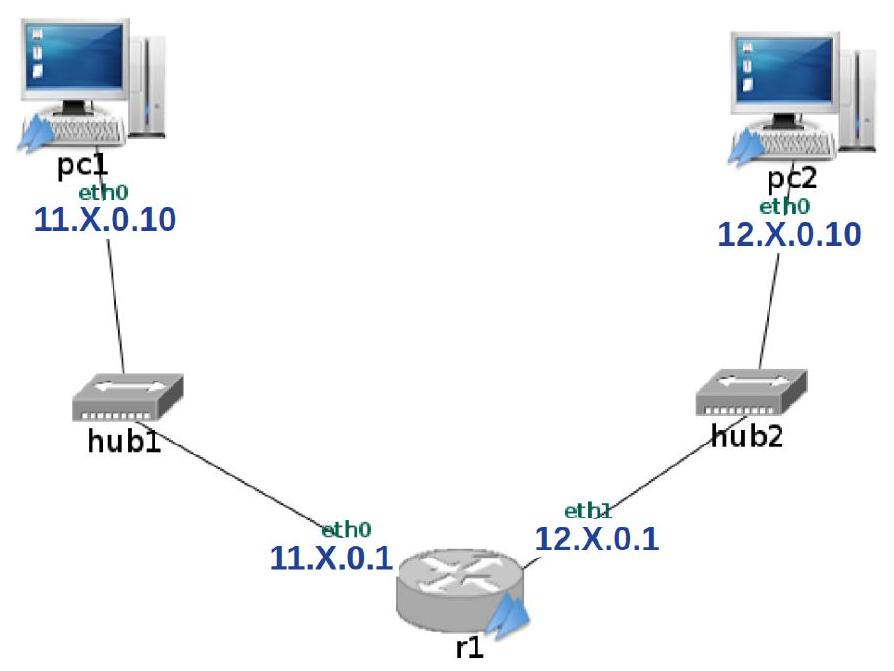
\includegraphics[max width=\textwidth]{enunciado1}
\end{center}

Arranca las máquinas de una en una, esperando que una máquina haya terminado su arranque antes de arrancar la siguiente.

En este apartado utilizarás la orden nc para observar el funcionamiento de UDP en diversas situaciones.

\subsection{UDP es un protocolo basado en datagramas: no hay establecimiento de conexión}
\begin{enumerate}
	\item Inicia una captura en el router $r 1$ (fichero de captura p5-udp-01.cap).
	
	\item Usando nc lanza una aplicación servidor UDP en la máquina pc2 y puerto 11111: nc -u -l -p 11111
	
	\item Usando nc lanza una aplicación cliente UDP en la máquina pc1 para que se comunique con el servidor (no envíes datos ni desde el cliente al servidor ni desde el servidor al cliente), desde el puerto local $33333:$ nc $-u$-p $33333<$ dir\_IP\_pc$>\ <$Pto\_destino$>$ 
	
	\item Interrumpe la captura.
	
\end{enumerate}

Explica qué paquetes deberían haberse capturado. Observa la captura y comprueba tu suposición.
\newline

No se ha capturado ningún paquete porque no se ha transmitido ningún mensaje entre servidor y cliente.

\subsection{Fragmentación IP con envíos UDP}
\begin{enumerate}
	\item Inicia una nueva captura en el router $r 1$ (fichero de captura p5-udp-02.cap).
	
	\item Escribe en el terminal donde tienes lanzado el cliente 20 líneas de texto, pulsando una letra cualquiera del teclado (con el tamaño por defecto del terminal de NetGUI, cada línea permite escribir 80 caracteres, así que estarás generando $80 \times 20=1600$ carácteres, cada uno de ellos ocupando 1 byte).
	
	\item A continuación pulsa la tecla INTRO o ENTER (véase la figura 2).
	
\end{enumerate}

\begin{center}
	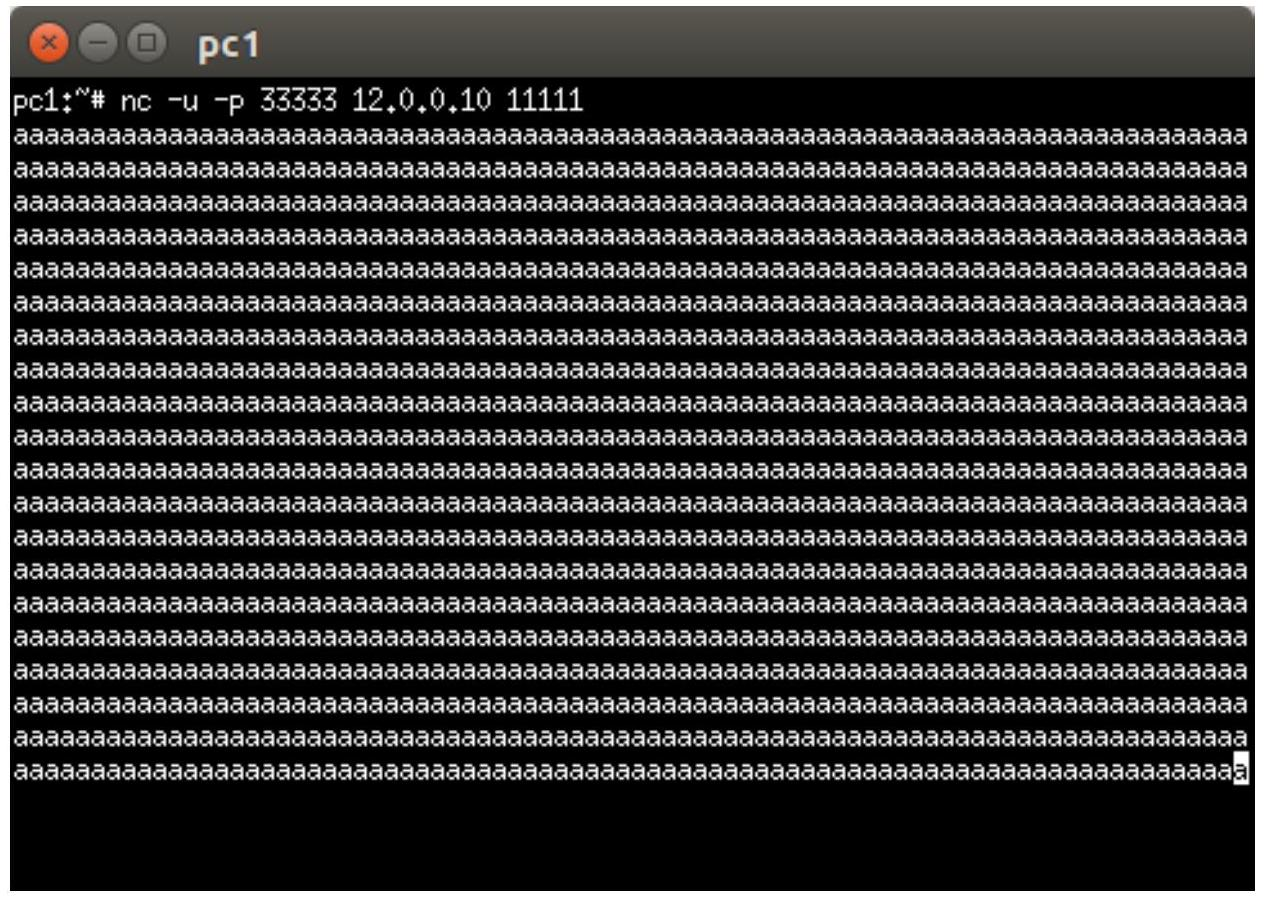
\includegraphics[max width=\textwidth]{enunciado2}
\end{center}

Antes de observar en la captura lo que ha ocurrido responde a estas preguntas:

\begin{enumerate}
	\item ¿cuántos datagramas UDP crees que se han enviado, y por qué?
	
	Se habrá enviado 2, porque el datagrama se fragmenta ya que es mayor a 1500 bytes
	
	\item ¿cuántos datagramas IP crees que se han enviado, y por qué?
	
	Se envían 2 también, debido a lo anterior
	
	\item ¿cuántos bytes de datos irán en cada datagrama UDP?
	
	En el primero irán 1480 bytes y en segundo irán el resto.
	
\end{enumerate}

Interrumpe ahora la captura y comprueba si tus suposiciones son correctas. Explica razonadamente el número de datagramas UDP, el número de datagramas IP, y el número de bytes de datos que va en cada uno de los datagramas UDP.

Se han enviado 2 datagramas IP que contienen mensajes UDP, el primero con 1480 bytes de datos, y el segundo con el resto.

\subsection{UDP es un protocolo basado en datagramas: no hay cierre de conexión}
\begin{enumerate}
	\item Inicia una captura en el router $r 1$ (fichero de captura p5-udp-03.cap).
	
	\item Interrumpe la ejecución del cliente pulsando Ctrl+C.
	
	\item Interrumpe la ejecución del servidor pulsando Ctrl+C.
	
\end{enumerate}

Piensa en cuántos paquetes deberían haberse capturado y por qué. Interrumpe la captura y comprueba tu suposición.

No recibe ningún mensaje, porque no envía ningún datagrama UDP

\subsection{Buffer de recepción en UDP}
Los protocolos de nivel de transporte trabajan tanto en TCP como en UDP con buffers in/out (recepción/envío) asociados a cada puerto (en el caso de TCP asociados a cada conexión). Cuando llega un datagrama UDP o un segmento TCP, se almacenan los bytes para la aplicación en el buffer in correspondiente. Cuando una aplicación envía bytes a través de un puerto UDP o de una conexión TCP, se almacenan sus bytes en el buffer out asociado a dicho puerto/conexión.

Para ver estos buffers vamos a utilizar la herramienta netstat.

\begin{enumerate}
	\item Inicia una captura en $r 1$ (guarda el contenido en el fichero p5-udp-04 . cap).
	
	\item Lanza en segundo plano ${ }^{1}$ una aplicación servidor utilizando nc en la máquina pc2 que reciba mensajes UDP destinados al puerto 11111 en segundo plano:
	
\end{enumerate}

$\mathrm{nc}-\mathrm{u}-1-\mathrm{p} \quad 11111$ \&

\begin{enumerate}
	\setcounter{enumi}{2}
	\item Observa el estado que muestra netstat - una en el servidor para la aplicación que acabas de arrancar y sus buffers.
	
	\item Trae a primer plano la ejecución de la aplicación servidor arrancada con nc, ejecutando para ello en el terminal del servidor esta orden: $f g$
	
\end{enumerate}

Tras traer a primer plano una aplicación, ésta recupera la entrada estándar del teclado. Ahora por tanto lo que se teclee se le envía a la aplicación servidor.

\begin{enumerate}
	\setcounter{enumi}{4}
	\item Pausa con Ctrl+Z la ejecución de la aplicación servidor nc. De esta forma la aplicación en el servidor siga arrancada pero no esté ejecutándose (la CPU no ejecutará instrucciones de la aplicación servidor mientras esté suspendida su ejecución). Mientras está suspendido el servidor, si la implementación de UDP en la máquina del servidor recibe datos destinados a la aplicación servidor, estos datos se almacenarán en el correspondiente buffer in, y no van a ser leídos por la aplicación nc porque su ejecución está suspendida temporalmente.
	
	\item Para ver cómo los datos se quedan almacenados en el buffer in de UDP del puerto en el que escucha el servidor, envía unos cuantos caracteres desde el cliente y pulsa la tecla INTRO o ENTER.
	
	\item Ejecuta netstat - una en el servidor para ver cómo esos datos se quedan en el buffer de recepción y no los lee la aplicación. Verás que la cantidad muestra 1712 bytes y no la cantidad de caracteres que has introducido desde el cliente. Esto es debido a que en UDP se reserva este cantidad en el buffer por cada paquete recibido.
	
	\item Ahora vamos a volver a activar el servidor, que estaba suspendido con Ctrl+Z, trayéndolo a primer plano. Ejecuta para ello la orden fg. Verás como inmediatamente los datos que habías enviado desde el cliente se muestran en la pantalla: la aplicación servidor los ha leído del buffer de recepción, que se ha vaciado, y los ha mostrado en la pantalla.
	
	\item Una vez realizada la prueba puedes interrumpir la ejecución del cliente y el servidor con Ctrl+C.
	
	\item Interrumpe la captura y trata de relacionar lo que ha ocurrido con el contenido de la captura.
	
	Recibe un solo datagrama UDP, que es lo que ocurriría si el servidor estuviera funcionando y no parado. 
	
\end{enumerate}

\subsection{Errores en las comunicaciones UDP}
Provoca las siguientes situaciones de error:

\begin{enumerate}
	\item Existe la máquina pc2, pero en ella no hay una aplicación servidor escuchando en el puerto 11111 . Inicia una captura en el router r1 (guarda el contenido en p5-udp-05. cap). Prueba a lanzar el cliente y envía datos desde el cliente. Interrumpe la captura. Explica razonadamente los paquetes capturados.
	
	Pc1 envía el datagrama UDP a pc2, que al recibirlo y no encontrar un servidor abierto en ese puerto envía un mensaje ICMP error 33 de vuelta a pc1
	
	\item Existe la red 12.X.0.0/24 y hay ruta para llegar hasta ella, pero no existe la máquina pc2 (para realizar este apartado apaga la máquina pc2). Inicia una captura en el router $r 1$ y guarda el contenido en p5-udp-06. cap. Prueba a lanzar el cliente y envía datos desde el cliente. Espera 1 minuto e interrumpe la captura. Explica su contenido.
	
	Pc1 envía el mensaje a la dirección Ip que anteriormente tenía pc2, pero como no sabe donde está, manda un datagrama ARP para encontrar esa dirección Ip a r1, y este al no encontrarla, manda un datagrama ICMP de error 31 de vuelta a pc1
	
\end{enumerate}

\chapter{Comunicación de aplicaciones usando el protocolo TCP}
En este apartado utilizarás la orden nc para observar el funcionamiento de TCP en diversas situaciones. Utilizaremos el mismo escenario NetGUI del apartado anterior.

${ }^{1}$ Añadiendo un carácter \& al final de una orden introducida en la shell se ejecuta dicha orden en segundo plano, lo que significa que la entrada del teclado no quedará ligada al proceso arrancado, pudiéndose así seguir ejecutando comandos en la shell a la vez que se está ejecutando concurrentemente la orden ejecutada en segundo plano

\section{TCP es un protocolo orientado a conexión.}
\subsection{Establecimiento de conexión}
\begin{enumerate}
	\item Inicia una captura en el router $r 1$ y guarda su contenido en un fichero (p5-tcp-01.cap).
	
	\item Usando nc, lanza una aplicación servidor en la máquina pc2 que atienda peticiones de conexión destinadas al puerto TCP 11111: nc -1 -p 11111
	
	\item Lanza una aplicación cliente con nc en la máquina pc1 para que se establezca una conexión TCP con la aplicación servidor, usando como puerto local TCP el 33333: nc -p 33333 <dir\_IP\_pc2> 11111. Explica cuántos paquetes deberían haberse capturado y por qué.
	
	Debería capturar tres datagramas TCP, ya que son los que se usan al iniciar la conexión. 2 irán desde pc1 a pc2, y 1 de pc2 a pc1 como respuesta del primero.
	
	Los primeros dos mensajes son para establecer la conexión, y el tercero es para indicarle a pc2 que le pueden llegar mensajes.
	
\end{enumerate}

Interrumpe la captura y comprueba si tus respuestas se corresponden con lo observado en la captura.

\subsection{Cierre de conexión}
\begin{enumerate}
	\item Inicia una captura en el router $\mathrm{r} 1$ y guarda el contenido en un fichero (p5-tcp-02.cap).
	
	\item Interrumpe la ejecución del cliente pulsando Ctrl+C en el cliente. Explica cuántos paquetes deberían haberse capturado y por qué.
	
	Se deberían haber capturado entre 3 o 4 paquetes, los dos primeros para notificar el fin de conexión y los últimos para asegurarlo.
	
\end{enumerate}

Interrumpe la captura y comprueba si tus respuestas se corresponden con lo observado en la captura.

NOTA: Con nc, una vez que se interrumpe la conexión desde el cliente, el servidor también cierra la conexión. Con otras aplicaciones podría mantenerse abierta la conexión desde el servidor si éste tuviera más datos que enviar.

\section{Buffer de recepción en TCP}
Vamos a visualizar los bufferes in/out (recepción/emisión) en TCP. Inicia una captura en el terminal de r1 guardando el contenido en un fichero (p5-tcp-03.cap).

\begin{enumerate}
	\item Lanza una aplicación servidor utilizando nc en la máquina pc2 que acepte conexiones en el puerto TCP 11111 (arráncala en segundo plano): nc - - $-p 11111$ \&
	
	\item Lanza una aplicación cliente con nc en la máquina pc1 para que se conecte al servidor, desde el puerto local TCP 33333: nc -p 33333 <dir\_IP\_pc2> 11111
	
	\item Observa el estado que muestra netstat - tna en el servidor y sus buffers.
	
	\item Trae a primer plano la ejecución de nc ejecutando en el terminal: fg
	
	\item Pausa con Ctrl $+Z$ la ejecución de nc en el servidor, para que la aplicación del servidor siga arrancada pero no se ejecute, por tanto, si TCP en el lado servidor recibe datos, estos no se se van a leer en nc quedarán almacenados en la cola de entrada de la implementación de TCP.
	
	\item Para ver cómo los datos se quedan almacenados en el servidor, envía una cadena de caracteres desde el cliente y pulsa INTRO.
	
	\item Ejecuta netstat - tna en el servidor para ver cómo esos datos se quedan en el buffer de recepción y no los lee la aplicación.
	
	\item Interrumpe la captura y fíjate cómo hay un asentimiento que indica que todos los datos han sido recibidos. Dado que la aplicación servidor está suspendida, los datos se encuentran almacenados en el buffer de recepción de la implementación de TCP, en el kernel del sistema operativo, pero no los ha leído aún la aplicación servidora arrancada con nc.
	
	\item Trae a primer plano la ejecución del servidor, para ello usa fg. Verás como los datos que habías enviado desde el cliente se muestran en la pantalla. El servidor los ha leído del buffer de recepción y el buffer está vacío.
	
	\includegraphics*[width=128mm, scale=0.5, center]{ejercicio1}
	
\end{enumerate}

Una vez realizada la prueba puedes interrumpir la ejecución del cliente y el servidor.

\section{Errores en las comunicaciones TCP}
Provoca las siguientes situaciones de error:

\begin{enumerate}
	\item Existe la máquina pc2 pero no hay una aplicación escuchando en el puerto 11111. Realiza una captura para comprobar el tráfico generado (p5-tcp-04.cap). Prueba a lanzar el cliente y comprueba qué ocurre.
	
	\includegraphics*[width=128mm, scale=0.5, center]{ejercicio2}
	
	\item Existe la red 12.X.0.0 y hay ruta para llegar hasta ella, pero no existe la máquina pc2. (Para realizar este apartado apaga la máquina pc2). Realiza una captura para comprobar el tráfico generado (p5-tcp-05.cap). Prueba a lanzar el cliente y comprueba qué ocurre. Interrumpe la captura y analízala.
	
	El protocolo TCP intenta crear la conexión con el servidor, pero al pasar el datagrama IP a r1, y este no poder enviarlo a pc2, envía de vuelta un mensaje ICMP de error 31 por cada mensaje TCP, es decir, 2 mensajes.
	
\end{enumerate}

\section{Análisis inicial de la captura de TCP}
En la captura tcp.cap se muestra una comunicación TCP entre dos aplicaciones.

Contesta a las siguientes preguntas:

\begin{enumerate}
	\item ¿Cuál es la dirección IP y el puerto del cliente TCP y la dirección IP y el puerto del servidor TCP?
	
	Cliente: Ip = 10.0.0.2 ; Puerto = 60709
	
	Servidor: Ip = 11.0.0.2 ; Puerto = 34000
	
	\item ¿Cuántos segmentos TCP se han enviado desde el cliente al servidor?
	
	Se han enviado 6 segmentos TCP
	
	\item ¿Cuántos segmentos TCP se han enviado desde el servidor al cliente?
	
	Se han enviado 4 segmentos TCP
	
	\item Indica qué extremo cierra antes la conexión.
	
	La conexión la cierra el cliente.
	
\end{enumerate}

\section{Números de secuencia}
Sigue analizando la captura tcp.cap.

Observa que, por defecto, Wireshark muestra números de secuencia relativos para los dos sentidos de la conexión. Seleccionando en el menú Edit $\rightarrow$ Preferences $\rightarrow$ Protocols $\rightarrow$ TCP, y desactiva la opción Relative Sequence Numbers. De esta forma podrás observar los números de secuencia reales, en lugar de los números relativos que muestra por omisión Wireshark. Deja de momento desactivada esta opción.

\begin{enumerate}
	\item ¿Cuáles son los números de secuencia reales que viajan en los paquetes que tienen activados el flag SYN o el flag FIN?
	
	Los números de secuencia para los mensajes con el flag SYN son: 1367801698 y 1363273423.
	
	Para los mensajes con el flag FIN son: 1367801710 y 1363273424
\end{enumerate}

Una vez que los hayas apuntado, vuelve a las opciones de TCP y activa otra vez la opción Relative Sequence Numbers. Compara ahora los números de secuencia relativos de los paquetes SYN y FIN.

Los números de secuencia para los mensajes con el flag SYN son: 0 y 0.

Para los mensajes con el flag FIN son: 12 y 1

Estos números relativos son la diferencia que había entre los números de secuencia anteriores.

Deja ya siempre activada la opción para ver los números de secuencia relativos ya que permite analizar más cómodamente la conexión.

NOTA: También puede resultarte conveniente desactivar la opción Ignore TCP Timestamps in Summary. De esta forma no aparecerán las marcas de tiempo (opción de TCP presente en los paquetes de algunas capturas) en el resumen de los paquetes, lo que te permitirá reconocer más rápidamente otros datos más importantes que figuran en ese resumen.

\begin{enumerate}
	\setcounter{enumi}{1}
	\item Fíjate en el campo Len que aparece en el resumen de los paquetes. ¿A qué se refiere?
	
	Se refiere a la cantidad de bytes de datos enviada desde el servidor al cliente o viceversa, pero solo se refiere a los datos del mensaje, no de todo el datagrama TCP.
\end{enumerate}

¿Cuántos bytes de datos envía el cliente al servidor? Si lo has calculado sumando los Len de los paquetes, ten en cuenta que algunos paquetes podrían ser retransmisiones (no pasa en esta captura) y no podrías sumarlos varias veces para calcular los bytes de datos enviados.

El cliente envía 11 bytes al servidor, porque es la cantidad resultante del offset final menos 1: 12 - 1 = 11 bytes\\

¿Cómo harías el cálculo si la conexión tuviera cientos de paquetes? Fíjate en el números de secuencia relativo del FIN que envía el cliente, y qué relación tienen con la cantidad de datos enviados.

Lo haría de la misma forma que en la pregunta anterior.\\


Ten en cuenta que el paquete FIN que envía el cliente podría contener datos, aunque eso no pasa en esta conexión. En ese caso, tendrías que tenerlos en cuenta también para calcular cuántos datos se envían en la conexión. Por esta razón es más conveniente es fijarse en el ACK del FIN que envía el servidor al cliente, ¿qué número de ACK lleva? ¿Qué relación tiene con la cantidad de datos enviados?

Tiene el valor 13, que es la suma del offset de la secuencia del cliente y la del servidor. La relación que tiene con la cantidad de datos enviada es similar a la del offset del cliente, pero en vez de restar 1, debes de restar 2 debido a las operaciones de inicio y cierre de conexión.

\begin{enumerate}
	\setcounter{enumi}{2}
	\item ¿Cuántos bytes de datos envía el servidor al cliente? Razona la respuesta en base a lo aprendido en la pregunta anterior.
	
	El servidor no envía ningún dato al cliente, ya que el offset de la secuencia del servidor es 1.
\end{enumerate}

\section{RTT}
Sigue analizando la captura tcp.cap.

\begin{enumerate}
	\item Para cada uno de los segmentos con datos que envía el cliente al servidor, para su paquete SYN y para su paquete FIN, indica cuál es el RTT del paquete. Observa para ello la columna Time del resumen de paquetes.
	
	SYN: RTT = 0.000134 s
	
	FIN: RTT = 4.170910 s
\end{enumerate}

\section{Retransmisión de SYN}
En la captura tcp-syn.cap se muestra una comunicación TCP. Contesta a las siguientes preguntas:

\begin{enumerate}
	\item ¿Cuántas veces se envía el segmento SYN del cliente al servidor? 
	
	Se envía 5 veces.
	
	\item Indica la secuencia de marcas de tiempo de los segmentos SYN enviados, y explica sus valores atendiendo al mecanismo exponential backoff. Ten en cuenta que al principio de una conexión aún no se ha podido medir el RTT del cliente al servidor. ¿Qué plazo de retransmisión inicial se ha utilizado ante la ausencia aún de un valor de RTT?
	
	1º mensaje: RTT = 0 s
	
	2º mensaje: RTT = 3 s
	
	3º mensaje: RTT = 9 s
	
	4º mensaje: RTT = 21 s
	
	5º mensaje: RTT = 45 s
	
	El mecanismo de \textit{exponential backoff} consiste en que cada vez que se retransmite el mismo paquete se dobla el plazo para ese paquete. El plazo de retransmisión inicial ha sido de 3 segundos.
	
	
	\item ¿Por qué crees que se ha retransmitido tantas veces el SYN? Observa los paquetes 8,10,12 y 14, ¿qué son? ¿Y los paquetes 9,11,13 y 15 ? ¿Cuál es por tanto la causa real de tantas retransmisiones del SYN?
	
	Se ha retransmitido tantas veces porque no era capaz de conectarse al servidor.\\
	Los paquetes 8,10,12 y 14 son las respuestas a la conexión que el servidor a enviado a modo de respuestas de esos SYN, pero estos están duplicados debido a que ya se ha iniciado la conexión debido al primer mensaje SYN del cliente.\\
	Los paquetes 9,11,13 y 15 son las respuestas del cliente a estos mensajes duplicados.\\
	La causa real de estos paquetes es el delay que existe entre el cliente y el servidor.
	
\end{enumerate}

\section{Funcionamiento básico de la ventana anunciada}
En la captura tcp-window . cap se muestra el principio de una comunicación TCP.

Ayudándote de la gráfica tcptrace, contesta a las siguientes preguntas relativas al sentido de comunicación 12.0.0.100:36185 $\rightarrow$ 13.0.0.100:37777:

\begin{enumerate}
	\item ¿Cuál es el número de secuencia del primer byte de datos contenido en el paquete número 6 ?
	
	Es 1
	
	\item ¿Cuál es el número de secuencia del último byte de datos contenido en el paquete número 6 ?
	
	Es 549
	
	\item El paquete número 8, ¿cuántos bytes de datos asiente? ¿cuál es el número de secuencia del último byte asentido por este paquete?
	
	Asiente 548 bytes, y el número de secuencia del último es 549
	
	\item Justo después de recibir el segmento número 8, y antes de recibir el segmento siguiente ¿cuál es el último valor de ventana anunciada por el receptor que ha recibido el emisor? ¿Cuántos bytes de datos podría enviar como máximo el emisor en ese momento, en uno o más segmentos, antes de que llegara otro ACK del receptor?
	
	El último valor de la ventana anunciada es 1097. Podría enviar 2593 bytes - 1097 bytes = 1496 bytes
	
	\item En el momento de enviar el paquete número 13, ¿en qué paquete venía la información de ventana aplicable al emisor en ese momento? ¿Cuántos bytes de datos más, además del paquete número 13, podría enviar el emisor en ese instante, antes de recibir otro ACK?
	
	La información venía en el paquete 9. Podría enviar 0 bytes más.
	
	\item ¿Podría haber enviado el emisor un segmento con datos nuevos en el instante 0.321000 segundos? ¿Por qué?
	
	No, porque no tenía información sobre la ventana anunciada.
	
	\item Identifica en la gráfica tcptrace de este sentido de la comunicación en qué otro periodo de tiempo se produce una situación similar a la que ocurre al enviarse el paquete número 13.
	
	Se produce en el paquete número 19.
	
\end{enumerate}

Cambia ahora el sentido de la comunicación sobre la gráfica tcptrace para analizar el sentido de comunicación 12.0.0.100:36185 $\rightarrow$ 13.0.0.100:37777:

\begin{enumerate}
	\item ¿Se envían bytes de datos en este sentido en los paquetes que hay en la captura? Compruébalo también sobre la lista de paquetes.
	
	No se envía ningún byte de datos.
\end{enumerate}

\section{Retransmisiones y asentimientos}
En la captura tcp-timeout-probes . cap se muestra el principio de una comunicación TCP.

Ayudándote de la gráfica tcptrace, contesta a las siguientes preguntas relativas al sentido de comunicación 12.0.0.100:43122 $\rightarrow$ 13.0.0.100:43123:

\begin{enumerate}
	\item El paquete número 16 es una retransmisión, aunque Wireshark no lo etiqueta como tal:

		\begin{enumerate}[label=\alph*]
			\item Mirando la gráfica tcptrace, ¿cómo puede identificarse que dicho paquete 16 es una retransmisión?
			
			\includegraphics*[width=128mm, scale=0.5, center]{ejercicio3}
			
			Se identifica porque no está en la posición siguiente al mensaje anterior y está en una posición en la que ya se ha transmitido un mensaje.
			\item ¿Qué paquete es la primera transmisión de los bytes de datos que viajan en el paquete 16 ?
			
			Es el paquete número 5
			\item ¿Cuál ha sido el plazo de retransmisión aplicado a esa primera retransmisión del paquete?
			
			Ha sido de 0.20935 segundos
			\item Mirando la gráfica tcptrace, ¿vuelve a ser retransmitido este paquete en la conexión? ¿Con qué plazo de retransmisión? ¿Por qué? Busca en la lista de paquetes la segunda retransmisión del paquete. Acostúmbrate a identificar paquetes en la gráfica y en la lista. Ayúdate del Time de los paquetes en la lista y de los valores de tiempo en el eje de las x de la gráfica.
			
			Vuelve a ser retransmitido en el paquete 18, con un plazo de retransmisión de 0.444351 segundos que es aporx. el doble debido al \textit{exponential backoff}.
			
			El paquete se reenvia debido a que no se encuentra la respuesta del servidor a ese mismo paquete.
		\end{enumerate}

	\item Identifica en la gráfica tcptrace otros segmentos que son retransmisión.
	
	Otro segmento que es retransmisión es el 45.
	
	\item En el momento de transmitir el paquete 18, ¿cuántos bytes están transmitidos y pendientes de que llegue su asentimiento? ¿Y cuántos paquetes (indica su número de paquete)?
	
	Se han transmitido 10136 bytes (7 paquetes) y falta el asentimiento de 8688 bytes (6 paquetes).
	
	\item El paquete 19 es un asentimiento. ¿Cuántos bytes asiente? ¿Y cuántos segmentos?
	
	Asiente 8688 bytes (6 paquetes).
	
	\item Identifica sobre la lista de paquetes otros asentimientos que asienten varios paquetes a la vez. Si utilizas la versión de wireshark-gtk verás que en la gráfica tcptrace se distingue cada paquete de asentimiento aunque lleguen varios casi a la vez. Así, con wireshark-gtk puede resultar más fácil identificar qué paquetes asiente cada asentimiento, cosa que no es tan fácil con la nueva versión de wireshark.
	
	El paquete número 26, 31, 36, 46, 54, 57, 63,
	
\end{enumerate}

\section{Sondas de ventana}
Sigue analizando la captura tcp-timeout-probes. cap. Responde a las siguientes cuestiones.

\begin{enumerate}
	\item Identifica en la gráfica tcptrace un periodo de tiempo en que el servidor está anunciando ventana 0 al cliente. Localiza en la lista de paquetes los que son enviados y recibidos en ese periodo de tiempo. ¿Por qué el cliente no envía bytes de datos en ese periodo de tiempo?
	
	Envía los paquetes del 63 al 67. El cliente no envía bytes de datos, porque al ser el tamaño de la ventana 0, no puede enviar bytes de datos.
	
	\item ¿Qué números de paquete son las sondas de ventana? ¿Cómo los etiqueta wireshark?
	
	Son los números 64, 66. Wireshark los etiqueta como TCP Keep-Alive
	
	\item ¿Cuánto tiempo pasa desde que el cliente recibe el primer anuncio de ventana 0 hasta que envía la primera sonda de ventana?
	
	Pasan 0.5 segundos
	
	\item ¿Cuánto tiempo pasa desde que el cliente recibe el segundo anuncio de ventana 0 hasta que envía la segunda sonda de ventana?
	
	Pasan 0.9 segundos
	
	\item ¿Qué paquete es el que anuncia al cliente que la ventana vuelve a estar abierta? ¿Cuántos bytes de datos puede enviar el cliente a partir de ese momento? ¿Entre qué números de secuencia?
	
	Lo anuncia el paquete número 68. El cliente entonces puede enviar 5792 bytes de datos, entre los números de secuencia 49233 y 55025
	
\end{enumerate}

\section{Factor de escala sobre la ventana anunciada}
Vuelve a abrir la captura tcp.cap.

En los segmentos que llevan activado el flag SYN se informa de los valores de número de secuencia inicial y ventana inicial anunciada que tiene cada extremo de la comunicación TCP. La opción factor de escala de la ventana (window scale), cuando se utiliza, se indica en la parte de opciones de los segmentos que llevan el flag SYN.

Cuando el lado que abre la conexión quiere utilizar un factor de escala para la ventana anunciada, activará la opción en su paquete SYN. El otro lado debe activar la opción en su paquete SYN+ACK para indicar que entiende esta opción de TCP y va a utilizarla también. A partir de este momento, en los segmentos que envíen ambos lados se aplicará el factor de escala para calcular el valor real de la ventana que se está anunciando: se multiplicará $2^{f a c t o r}$ por el campo de ventana anunciada que viaja en el segmento. Nótese que sólo en el segmento SYN y en el SYN+ACK viaja el factor de escala, pero éste no se aplica al campo ventana anunciada de estos dos segmentos, sino que se aplica a todos los demás segmentos enviados.

\begin{enumerate}
	\item Observa los segmentos SYN enviados por el cliente y por el servidor. En el segundo panel de Wireshark despliega la cabecera TCP y busca la parte de opciones. Localiza la opción Window Scale. Indica el factor de escala que envía el cliente y el factor de escala que envía el servidor.
	
	El factor de escala que envía el cliente es 2, y el del servidor es 2.
\end{enumerate}

Observa que en el resumen de paquetes, para los paquetes SYN Wireshark anota WS= $\mathrm{x}$ siendo $\mathrm{x}=2^{\text {factor }}$.

Mira dentro la cabecera de los dos paquetes SYN el campo de ventana anunciada. Observa que Wireshark muestra el valor real del campo (Window size value) y luego el valor tras aplicar el factor de escala Calculated window size. Observa que en los paquetes SYN aún no se aplica el factor de escala.

\begin{enumerate}
	\setcounter{enumi}{1}
	\item Indica cuál es el valor del campo de ventana anunciada (Window size) en el resto de los segmentos de la conexión (los que NO tienen el flag SYN activado) en cada uno de los dos sentidos.
	
	El valor de Window size es de 2920 para el cliente y 2896 para el servidor, y el valor escalado es de 5840 y 5792 respectivamente.
\end{enumerate}

Observa que en el resumen de paquetes aparece el valor de ventana ya escalado, mientras que en la cabecera puedes comprobar el valor que viaja en el campo, y el valor tras aplicar el escalado.

Señala para cada paquete el valor que viaja en el campo y el valor final de la ventana anunciada tras aplicar el factor de escala.

Ten en cuenta que en esta captura los lados utilizan el mismo factor de escala, pero en otras conexiones cada lado podría usar un factor de escala diferente para sus valores de ventana.

NOTA: En muchas conexiones podrás ver que las ventanas anunciadas inicialmente son relativamente pequeñas, y que poco a poco, según avanza la conexión y el emisor va enviando datos, el receptor le aumenta el tamaño de ventana. Esto se debe a que la implementación de TCP comienza reservando un buffer de recepción no demasiado grande, porque no sabe si el emisor va a transmitir muchos o pocos datos. Según el emisor va llenando la ventana, el receptor (si dispone de más memoria) va aumentando el tamaño del buffer, y por lo tanto, de la ventana anunciada.

\section{MSS}
En la captura tcp-mss-pmtu.cap se muestra el principio de una comunicación TCP. Ordena en Wireshark los paquetes por la columna Time. Contesta a las siguientes preguntas:

\begin{enumerate}
	\item Indica cuál es el valor anunciado de MSS en la parte opcional de las cabeceras de los paquetes SYN de los dos sentidos de la conexión. Dados estos dos valores, indica qué tamaño de datos crees usarán ambos sentidos de la conexión si tienen que enviar datos.
	
	En el cliente es de 660 y en el servidor es de 560. El tamaño de bytes de datos que enviarán será de 520 y 620 resectivamente.
	
	\item Mira los tamaños de las cabeceras de los segmentos 1 y 3 enviados por el cliente y verás que son distintos. Teniendo en cuenta que cada segmento enviado en la conexión podría tener un tamaño de cabecera diferente, ¿cómo se calculará la cantidad máxima de datos que puede llevar un segmento dado el MSS y el tamaño de la cabecera?
	
	El tamaño se calcula omitiendo las opciones de TCP, por lo que ambos mensajes tendrán el mismo MSS. El máximo número de bytes de datos se calcula restándole al MSS la cabezera Ip (20) y la cabecera TCP (20) sin opciones.
	
	\item Teniendo en cuenta que en el instante en el que se envía el segmento número 4, la máquina 11.0.0.11 tenía más de $2.000$ bytes de datos que enviar a la máquina 12.0.0.12, ¿por qué envía menos? ¿Cuántos bytes envía en ese segmento 4 ? ¿Cómo se justifica el número de bytes de datos que contiene el segmento 4 dados los valores de MSS anunciados en los segmentos SYN?
	
	En el segmento 4 envía 548 bytes de datos, porque al superar el mensaje a enviar el MSS del servidor, se debe de fragmentar en dos mensajes de menor tamaño.
	
	\item Explica qué tipo de paquete son los paquetes 5 y 7 de la captura. ¿Qué significan y cuál puede ser la razón de que se hayan enviado? ¿Qué campo de la cabecera IP de los paquetes 4 y 6 ha provocado que se envíen los paquetes 5 y 7 ?
	
	Los paquetes 5 y 7 de la captura son la respuesta del servidor a los paquetes 4 y 6. Como la longitud de estos paquetes supera el MSS del servidor, este envía un datagrama ICMP de error 34 para indicarle al cliente que debe fragmentar los paquetes.
	
	\item Mira el paquete 8 de la captura. ¿Por qué se retransmite este segmento? Comprueba el tamaño de su campo de datos. Explica la relación de este valor con la información contenida en los paquetes 5 y 7 .
	
	El paquete número 8 y 9 es la retransmisión del paquete 4 pero fragmentado de una forma que el MSS del servidor lo acepte.
	
\end{enumerate}

\end{document}